% 2011 年陕西卷文科第 4 题：y=x^(1/3) 的图象（四选一）。
% 来源 PDF：普通高考/2011/2011陕西文.pdf，SHA-256 ae7984faa1d48b19525f0991a1795d8ea34b7ac65d9c067f4862c59ae112880e。
% 原页：第 1 页第 1 栏下部，书页码 695。虚线为 y=x。
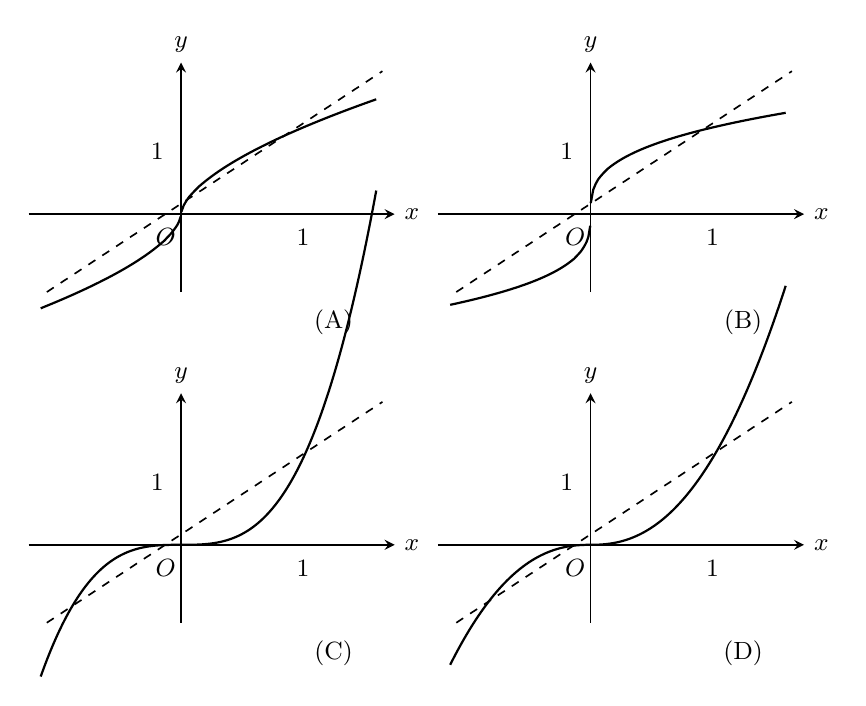
\begin{tikzpicture}[>=stealth, semithick, font=\small]
  \foreach \dx/\dy/\lab/\p in {0/0/A/0.6, 5.2/0/B/0.3333, 0/-4.2/C/3, 5.2/-4.2/D/2.3333} {
    \begin{scope}[shift={(\dx,\dy)}, xscale=1.55, yscale=1.1]
      \draw[->] (-1.25,0)--(1.75,0) node[right] {$x$};
      \draw[->] (0,-0.9)--(0,1.75) node[above] {$y$};
      \draw[dashed] (-1.1,-0.9)--(1.65,1.65);
      \draw[thick, domain=-1.15:-0.002, samples=80] plot (\x,{-pow(-\x,\p)});
      \draw[thick, domain=0.002:1.6, samples=80] plot (\x,{pow(\x,\p)});
      \node[below left] at (0.04,-0.05) {$O$};
      \node[left] at (-0.06,0.72) {$1$};
      \node[below] at (1.0,-0.06) {$1$};
      \node at (1.25,-1.25) {(\lab)};
    \end{scope}
  }
\end{tikzpicture}
